\section{General}




\subsection{Conventions}
3D graphics APIs usually all have their own conventions regarding coordinate systems, vector and matrix forms, and so on. It is therefore imperative for a 3D framework to have well defined conventions that are used throughout. This section outlines the conventions used in the PixelLight renderer API.

The renderer component uses the right hand system - matrices are column major order like OpenGL does, but unlike Direct3D, x points to right, y upward and z points to the eye. (see figure below) The vertices of front faces are specified in counter clockwise winding. Therefore, backface culling will usually be set to cull clockwise-oriented faces.

\begin{figure}
  \centering
  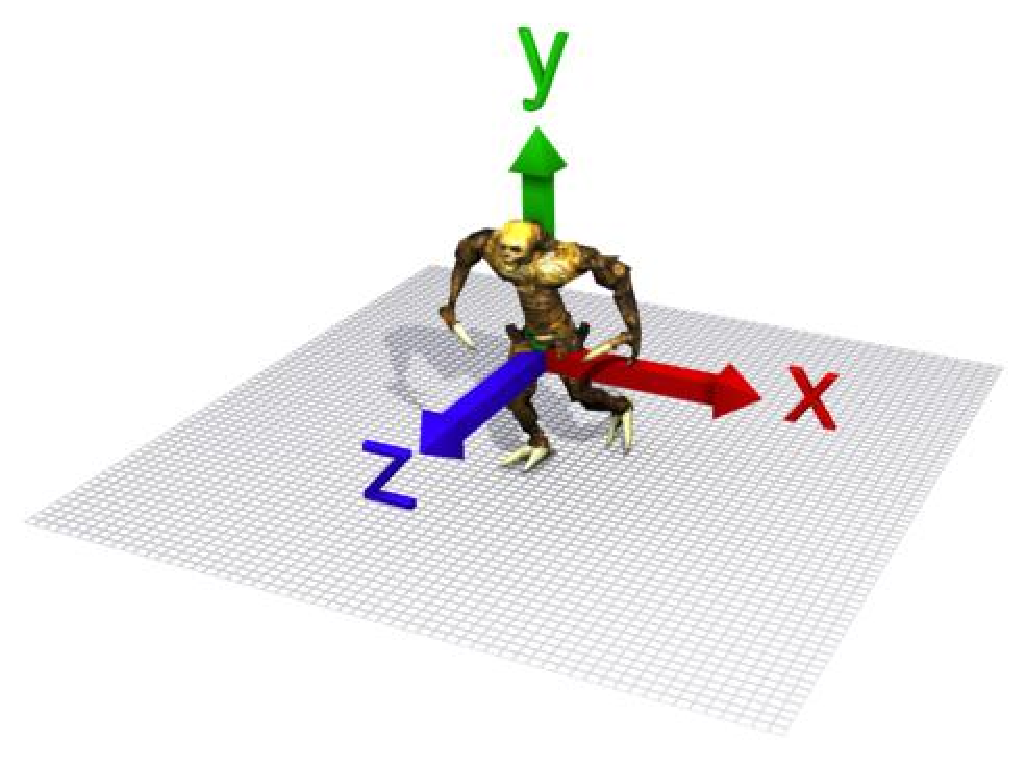
\includegraphics[scale=0.7]{pics/CoordinateSystem.eps}
  \caption{Coordinate system}
  \label{fig:Coordinate system}
\end{figure}

In the PixelLight framework itself scene nodes use the z axe as direction vector, x as left and y as up-vector. Cameras and spot lights invert the \emph{natural} z-axis internally so they can be used in the same way as all other scene nodes without the need to rotate them around 180 degrees along the y-axis - but this components are unknown at this level so we don't go into details in here.




\subsection{Renderer Component High-Level Class Diagram}
The following class diagram shows a high-level view of the most important class hierarchies in the render system, in particular the hierarchy of render resource, render surface and state classes. The subsequent sections describe the most important classes in more detail. The diagram is split up into three parts. The renderer itself, the API backends the user will not use directly and and examples how the framework is using some renderer classes in general.

\begin{figure}
  \centering
  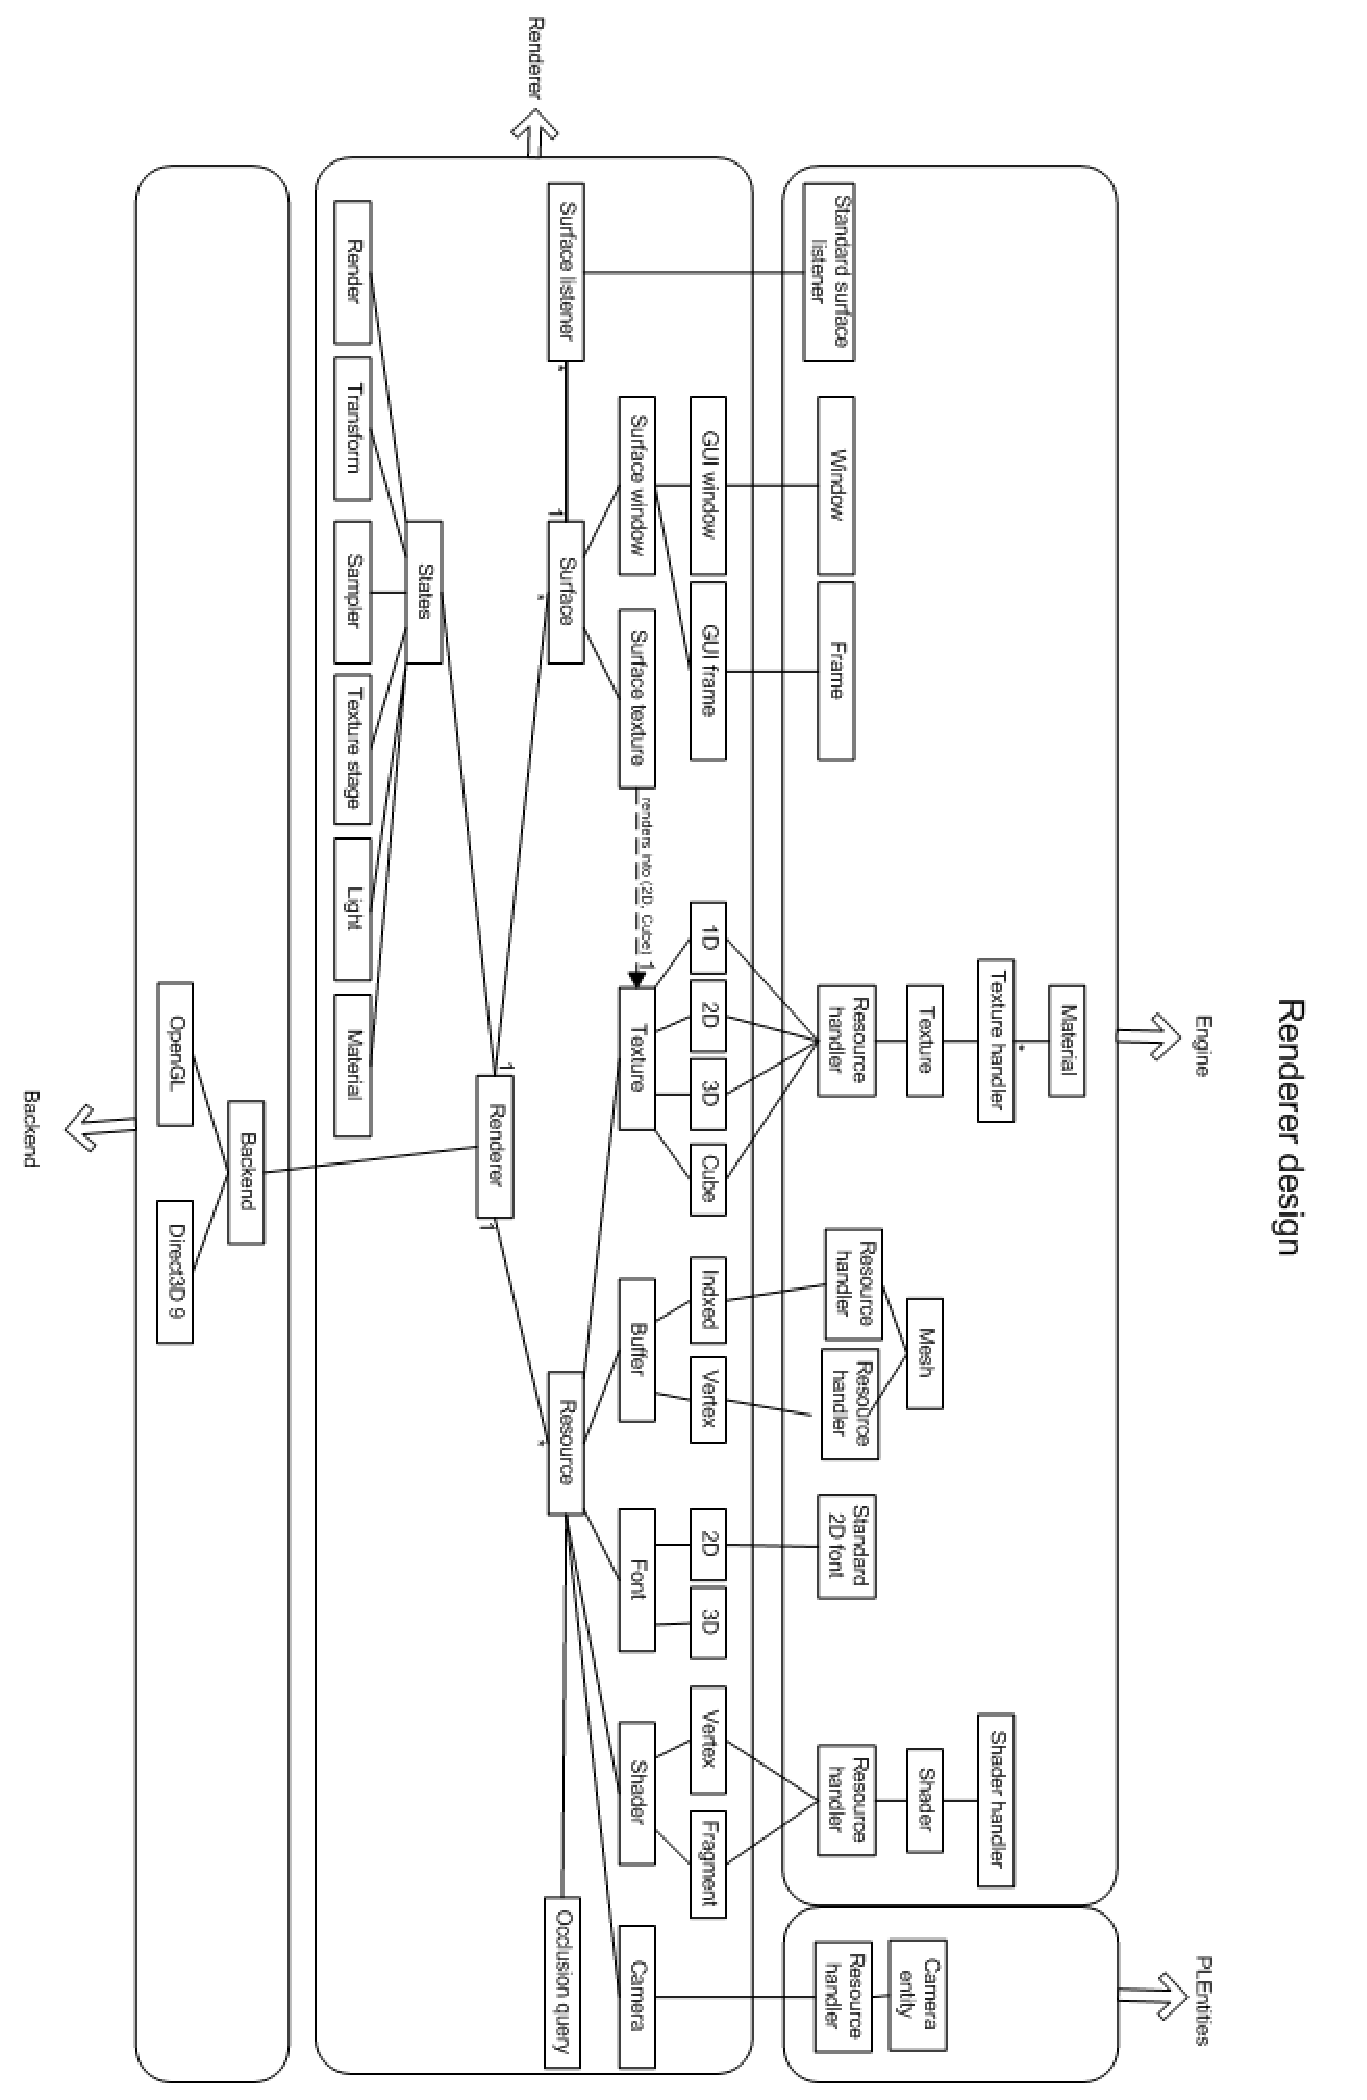
\includegraphics[scale=0.7]{pics/PLRendererClassDiagram.eps}
  \caption{Renderer component}
  \label{fig:Renderer component high-level class diagram}
\end{figure}




\subsection{Renderer Instance}
With the interface of the created renderer instance, an application can begin and end a scene, swap back with front buffers, create render targets (different types of windows and textures) and render resources, draw primitives, set render states etc. There's also a function to set the world, view and projection matrices and a whole range of other methods that usually directly map to the underlying rendering API. One of the most frequently called methods of the renderer system are the two draw methods used to render primitives to the currently active render target. Supported primitives are point lists, line lists, line strips, triangle lists, triangle strips, and triangle fans. The vertices that compose primitives are stored in a vertex buffer. One of the draw methods takes a vertex buffer as input parameter and renders the geometry contained in the vertex buffers defined by the mapping to the current render target. Another draw method additionally takes an index buffer as input parameter and renders indexed primitives to the current render target. It is advisable to use indexed primitives whenever possible, because it reduces the amount of memory sent to the graphics hardware. With indexed primitives, multiple primitives can use the same vertex by reusing its index in the index buffer buffer without having to duplicate all the vertex attributes of that vertex in the vertex buffer.

The renderer classes are actually abstract base classes which classes are derived in the renderer backends that implement most of the functionality using the underlying rendering API. Most of the time, the deriving classes have to map the routines to the corresponding routines of the rendering API and not actually implement much. Therefore, implementing a renderer for a new 3D graphics API is usually a task that is tedious, because of the high number of routines to implement, uncomplicated, since it mostly only involves mapping functions to functions - but headache producing when it comes to hardware dependent irregularities that are often not obvious by just looking at the code and that are not reproducible on each hardware and driver version. But it's also a bit tricky because in some cases the different APIs are quite different. Direct3D has some special features OpenGL has not, OpenGL has some special features Direct3D has not - therefore, in the most cases, the PixelLight renderer ONLY supplies things BOTH API's have. No \emph{glVertex}... calls, quad primitives etc. because Direct3D does not have these things.




\subsection{Additional Tool Functions}
Within the PixelLight renderer, there are a few special tool functions which are normally not within the native renderer API's like OpenGL - but they will make your life more comfortable. There are some 2D functions you can for instance use for an ingame gui - or for 2D games.

Using \emph{Begin2DMode()} you begin the 2D mode and a orthogonal projection matrix is set automatically. Now you can draw your images using \emph{DrawImage()}, draw some points, lines, texts etc. By calling \emph{End2DMode()} you return into the previous \emph{3D mode}.

There are also some additional draw functions like \emph{DrawBox()} you can use to visualize some debugging stuff. This functions don't offer that many settings - they are for debugging only. To draw more complex stuff, fill the vertex and index buffers by self or use the PixelLight mesh library which can also create a lot of geometric meshes automatically.



\subsubsection{Renderer Resources and States}
Nearly most of the renderer interfaces are dealing with resources and states. In the section \emph{Renderer component high-level class diagram} you can see the different types of resources and states. By using functions like \emph{CreateTextureBuffer2D()} you create such resources, by using state functions like \emph{SetRenderState()} you can set, get etc. states. If you are familiar with Direct3D you shouldn't have any problems by using the PixelLight renderer. For OpenGL users this may be unaccustomed to set for instance all the different render states using ONE function \emph{SetRenderState()} - but this way is more handy, especial if you want to backup/restore all states at once.\footnote{OpenGL has push/pop state functions, but they are not that comfortable}



\subsubsection{Vertex and Index Buffers}
All geometry data submitted to the renderer component must be stored in vertex and index buffers which are derived of a basis buffer. A vertex buffer stores vertices where a vertex has a number of vertex attributes, such as position, normal, color, and so on. An index buffer stores indices into a vertex buffer pointing to certain vertices. To actually draw the geometry data, one of the draw methods of the renderer must be called. The draw methods take the primitive type, such as line list or triangle strip, and the number of primitives that are to be rendered as input parameters. One draw method just requires a vertex buffer as parameter containing all the vertices that define the to-be-drawn primitives. The vertices in the buffer are used one after the other. If, for example, the given primitive type is triangle list, every three vertices of the vertex buffers will be used to render a triangle. Another draw method also takes a vertex buffer as input parameter and additionally an index buffer which contains indices into the vertex buffer adding a level of indirection. If the specified primitive type is again triangle list, every three indices in the index buffer will be used to retrieve three vertices from the vertex buffer that are then used to render a triangle. Since both vertex and index buffer are render resources, they can potentially be stored in video memory. When allocating a buffer you have to define it's usage, if it is static, dynamic etc. this definition will help the renderer to store the data in a optimal memory section. Static buffers normally directly stored on the 
memory of the GPU which is quite performant.

By defining \emph{vertex attributes} you specify the layout of a single vertex... that apply to ALL vertices within the vertex buffer. There are multiple \emph{semantics}, \emph{channels} and \emph{types} an attribute can choose from. The semantic defines the \emph{usual} usage of the attribute. Within a \emph{Position} attribute \emph{normally} a vertex position is stored - but when using shaders you can store everything within every semantic, but we recommend to respect some guidelines. Some semantics can have multiple channels, the \emph{TexCoord} semantic for example for multitexturing or providing additional data for shaders that do not fit into any other semantic.

Here's an excerpt from possible semantics:
\begin{itemize}
\item{Position}
\item{Normal}
\item{Color[n]}
\item{TexCoord[n]}
\end{itemize}

\emph{Color[n]} specifies n sets of colors, were the first is normally the primary color and the second the secondary color. \emph{TexCoord[n]} specifies n sets of texture coordinates, where n is a zero-based texture sampler stage index and cannot be greater than the number of available stages.

The attribute \emph{type} specifies the structure of the concrete attribute data - \emph{Float3} is for example quite common to store the x, y and z components of a vertex position. For the fixed-function pipeline the meaning and type of the vertex attributes is fixed and cannot be modified. But today you only need to take this into consideration when developing for legacy or minimal hardware. Vertex attributes are added using the vertex buffer method \emph{AddVertexAttribute()}. Normally you first setup all vertex attributes before allocating the buffer itself, but its possible to also add vertex attributes AFTER a buffer was allocated, but normally this isn't recommended for performance reasons.

The vertex attribute sets do not have to be ordered neither for fixed-function nor for programmable pipeline. So this would be a perfectly legal binding for the pipeline:\\
Normal - TexCoord[2] - Position - TexCoord[0] - TexCoord[1]\\
... but none we personally would use.

Before manipulating or reading of a vertex or index buffer you have to call \emph{Lock()} were you should define what you want to to with the buffer - reading, writing etc. After your operations on the buffer are done you have to call the \emph{Unlock()} function. Try to avoid manipulating the buffers often per frame. Use the \emph{GetData()} function of the buffer to get the desired data. When working on vertex buffers you have to define WHAT you want to edit. When accessing colors you should use the special color functions. You should NEVER see the vertex buffer as a normal well defined linear buffer were you know how many bytes each vertex attributes will have etc. because for instance different API's will manage the colors in a different way. Using this provided vertex buffer function you don't have to care about this API dependent stuff yourself and you are always on the safe side.



\subsubsection{Occlusion Query}
This defines a mechanism whereby an application can query the number of pixels, or more precisely samples, drawn by a primitive or group of primitives.

The primary purpose of such a query, hereafter referred to as an \emph{occlusion query}, is to determine the visibility of an object. Typically, the application will render the major occluders in the scene, then perform an occlusion query for the bounding box of each detail object in the scene. Only if said bounding box is visible, i.e., if at least one sample is drawn, should the corresponding object be drawn.

Here some examples were it's useful to know how many fragments of an object are visible:
\begin{itemize}
\item{Objects that are visible but cover only a very small number of pixels can be skipped at a minimal reduction of image quality.}
\item{Knowing exactly how many pixels an object might cover may help the application decide which level-of-detail model should be used. If only a few pixels are visible, a low-detail model may be acceptable.}
\item{Occlusion queries can replace read functions of the depth buffer to determine whether, for example, a light source is visible for the purposes of a lens flare effect or a halo to simulate glare. Pixel counts allow you to compute the percentage of the light source that is visible, and the brightness of these effects can be modulated accordingly.}
\end{itemize}




\subsection{Rectangle Textures}
\hypertarget{Rectangle textures}{}
Lookout, this section is only relevant for legacy GPU's/drivers. Nowadays, the power-of-two dimension restriction for textures is gone. If you don't care about support for legacy hardware without universal NPOT, just skip this section.

In past days, the hardware texturing was limited to images with power-of-two dimensions and an optional 1-texel border. But there was also a special kind of textures called \emph{rectangle textures} without requiring power-of-two dimensions.

Non-power-of-two dimensioned textures are useful for storing video images that do not have power-of-two dimensions - for instance the most ingame gui elements. Re-sampling artefacts are avoided and less texture memory may be required by using non-power-of-two dimensioned textures. Non-power-of-two dimensioned textures are also useful for shadow maps and window-space texturing.

However, non-power-of-two dimensioned (NPOTD) textures have limitations that do not apply to power-of-two dimensioned (POT) textures. NPOTD textures may not use mipmap filtering; POTD textures support both mipmapped and non-mipmapped filtering. NPOTD textures support only the CLAMP, CLAMP TO EDGE, and CLAMP TO BORDER wrap modes; POTD textures support CLAMP TO EDGE, REPEAT, CLAMP, MIRRORED REPEAT, and CLAMP TO BORDER. NPOTD textures do not support an optional 1-texel border;
POTD textures do support an optional 1-texel border.

Whether a texture is a rectangle texture or not is defined in the textures \emph{plt}-file:

\begin{lstlisting}[caption=\emph{plt}-file rectangle texture setup]
<?xml version="1.0"?>
<Texture Version="1">
    <General Rectangle="1" />
</Texture>
\end{lstlisting}

Were the default value is 0 meaning that by default all textures must have a power-of-two dimension! If no rectangle textures are supported by the renderer, this setting will have no effect and power-of-two are used.




\subsection{Texture Compression}
Try to use texture compression whenever possible - this will shorten the loading times, enhance the performance and of course, will safe memory on the GPU. The \emph{dds} image file format is best suited for this task because it supports many texture compression formats a GPU's can directly work with. Other traditional image file formats like \emph{jpg} should not be used as texture - GPU's don't understand the used compression techniques, and therefore after loading such an image, the data needs to be decompressed on the CPU in order to be able to upload it to the GPU. This is a slow process resulting in images with compression artefacts, but without a usable compression - it's even worse if this uncompressed data is compressed for instance to \emph{DXT1}\footnote{Called \emph{BC1} in \emph{DirectX 10}} before uploading to the CPU. (slow and additional compression artefacts)

During production, one can use uncompressed textures so no compression artefacts are introduces during production when manipulating a texture multiple times. When publishing something, we highly recommend that the textures are compressed in a proper way. The additional work is really worth the effort, belief us.


\paragraph{Luminance Map Compression}
When using luminance maps, meaning maps with only one channel, \emph{LATC1}\footnote{Called \emph{BC4} in \emph{DirectX 10}, formerly \emph{ATI1N} on ATI GPU's only} is a good choice for texture compression with high quality and the same memory footprint as \emph{DXT1}.


\paragraph{Color Map Compression}
When using color maps like photos, meaning maps with three channels, \emph{DXT1} is a good choice for texture compression.


\paragraph{Color Map with Alpha Channel Compression}
When using color maps which contain a alpha channel, meaning maps with four channels, \emph{DXT5}\footnote{Called \emph{BC3} in \emph{DirectX 10}} is a good choice for texture compression. For alpha channels with low coherency, \emph{DXT3}\footnote{Called \emph{BC2} in \emph{DirectX 10}} may reduce the memory footprint while still having a acceptable quality.


\paragraph{Normal Map Compression}
In general, do never ever compress normal maps with standard compression formats like \emph{DXT1}, \emph{DXT3} or \emph{DXT5}, this will lead to ugly visible normal artefacts because this formats are optimized for color based data, but in this case, we have vector data stored in the texture! \emph{DXT5 xGxR} can be used for best backward compatibility (not the best quality) and \emph{LATC2}\footnote{Called \emph{BC5} in \emph{DirectX 10}, formerly \emph{3DC}/\emph{ATI2N} on ATI GPU's only} is the recommended format for normal map compression with reasonable quality and the same memory footprint as \emph{DXT5}. PixelLight also supports \emph{Alternate XY Swizzle LATC2} which enables shader code reuse of \emph{DXT5 xGxR}.

\emph{DXT5 xGxR} and \emph{Alternate XY Swizzle LATC2} are no standard extensions of the \emph{dds} image file format. Tools like \emph{The Compressonator} usually store their own additional information within the file to mark the special format, but other tools can't read in and understand this information. Instead of manipulating the \emph{dds} image file format, we decided to add an optional \emph{plt}-file per texture to add additional information about a texture.

To mark a texture as \emph{DXT5 xGxR}, add a \emph{plt}-file with the same name as the texture and with the following content:
\begin{lstlisting}[caption=\emph{plt}-file \emph{DXT5 xGxR} normal map compression]
<?xml version="1.0"?>
<Texture Version="1">
    <General Compression="DXT5_xGxR" />
</Texture>
\end{lstlisting}

To mark a texture as \emph{Alternate XY Swizzle LATC2}, add a \emph{plt}-file with the same name as the texture and with the following content:
\begin{lstlisting}[caption=\emph{plt}-file \emph{Alternate XY Swizzle LATC2} normal map compression]
<?xml version="1.0"?>
<Texture Version="1">
    <General Compression="LATC2_XYSwizzle" />
</Texture>
\end{lstlisting}


\paragraph{More Information and Tools}
For additional information about texture compression, especially about normal map compression, have a look at 
\url{http://developer.nvidia.com/object/real-time-normal-map-dxt-compression.html} and \url{http://www.ozone3d.net/tutorials/bump_map_compression.php}.
There are many tools dealing with textures, \emph{The Compressonator}\footnote{\url{http://developer.amd.com/gpu/compressonator/Pages/default.aspx}} from ATI is one of the better ones and can directly deal with for instance \emph{DXT5 xGxR} or \emph{Alternate XY Swizzle LATC2}.
